% ============================================================ the paper in a nutshell
\section{The paper}

\begin{frame}{The review}
  \begin{columns}[c]
    \column{0.40\textwidth}
    \centering
    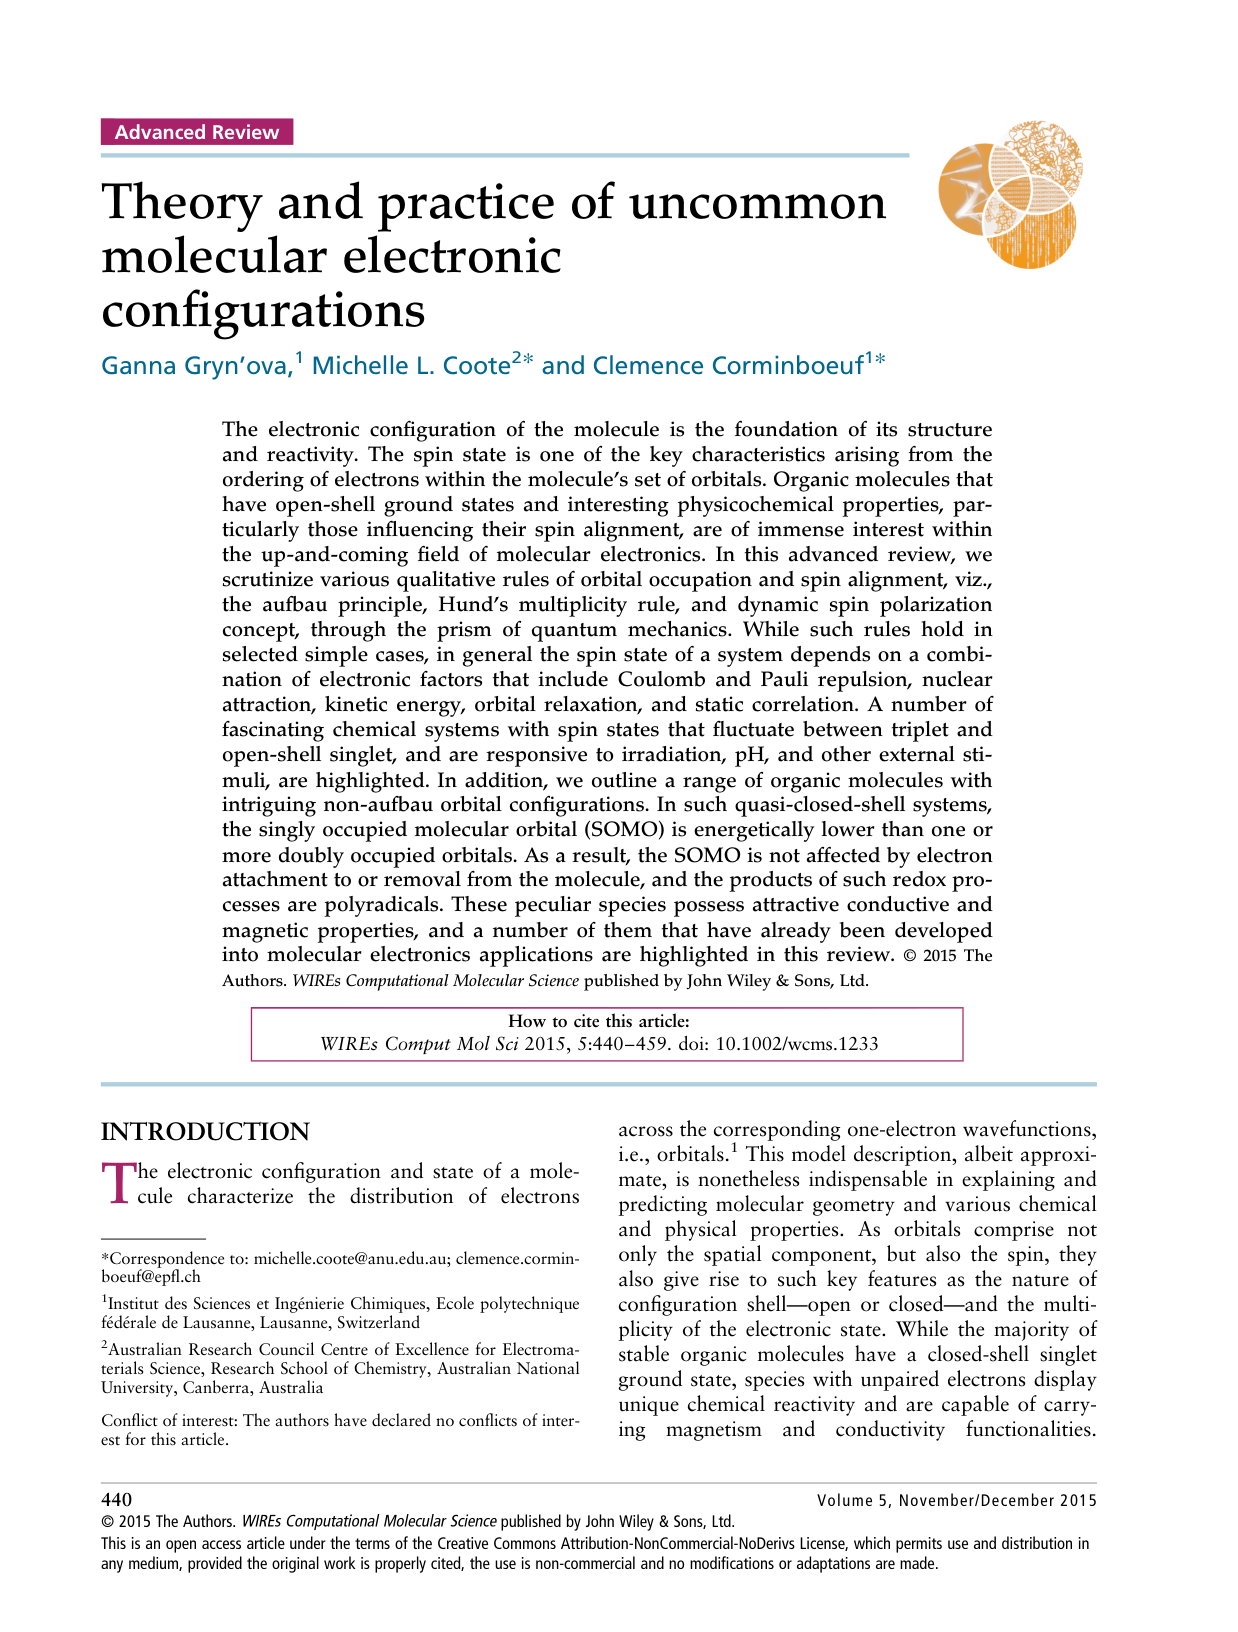
\includegraphics[height=0.74\textheight]{screenshots/paper_page1.png}
    \column{0.58\textwidth}
    {\noircalli\Large\cgold{Theory and practice of uncommon\\ molecular electronic configurations}}
    \vskip0.3cm
    {\noirgaramond Ganna Gryn'ova, Michelle L.\ Coote, Cl\'emence Corminboeuf}
    \vskip0.2cm
    {\small\cmuted{\emph{WIREs Computational Molecular Science} \textbf{5}, 440--459 (2015)\\
      doi:10.1002/wcms.1233 \quad Advanced Review, open access}}
    \vskip0.4cm
    \begin{itemize}
      \item<2-> 20 pages, 17 figures, 5 schemes, 118 references
      \item<3-> part theory (what decides a spin state?)
      \item<4-> part catalogue (molecules that break the textbook rules)
    \end{itemize}
  \end{columns}
\end{frame}

\begin{frame}{Two uncommon configurations}{the two halves of the paper}
  \begin{columns}[T]
    \column{0.48\textwidth}
    \centering{\gsc{1.\ fluctuating multiplicity}}\par\vskip0.2cm
    \begin{tikzpicture}[scale=1.55]
      \begin{scope}
        \orblevel{0}{0}{} \orblevel{0}{0.18}{}
        \elup{0}{0}\elup{0}{0.18}
        \node[font=\scriptsize,text=noirrose] at (0,-0.55) {triplet};
      \end{scope}
      \node[font=\large,text=noirgold] at (1.25,0.1) {vs};
      \begin{scope}[xshift=2.5cm]
        \orblevel{0}{0}{} \orblevel{0}{0.18}{}
        \elup{0}{0}\eldn{0}{0.18}
        \node[font=\scriptsize,text=noirblue] at (0,-0.55) {open-shell singlet};
      \end{scope}
    \end{tikzpicture}
    \vskip0.2cm
    \small two (nearly) degenerate orbitals, two electrons:\\
    \emph{parallel} or \emph{antiparallel}? \\[2pt]
    \onslide<2->{\cgold{Who wins: Hund's rule, or correlation?}}
    \column{0.48\textwidth}
    \centering{\gsc{2.\ non-aufbau ordering}}\par\vskip0.2cm
    \begin{tikzpicture}[scale=1.55]
      \begin{scope}
        \orblevel{0}{1.0}{} \orblevel{0}{0.5}{SOMO} \orblevel{0}{0}{}
        \elup{0}{0.5}\elup{0}{0}\eldn{0}{0}
        \node[font=\scriptsize,text=noirmuted] at (0,-0.55) {aufbau};
      \end{scope}
      \begin{scope}[xshift=2.6cm]
        \orblevel{0}{1.0}{} \orblevel{0}{0.5}{HOMO} \orblevel{0}{0}{SOMO}
        \elup{0}{0.5}\eldn{0}{0.5}\elup{0}{0}
        \node[font=\scriptsize,text=noirrose] at (0,-0.55) {quasi-closed shell};
      \end{scope}
    \end{tikzpicture}
    \vskip0.2cm
    \small the singly occupied orbital lies \emph{below}\\ a doubly occupied one \\[2pt]
    \onslide<3->{\cgold{Oxidation then makes a diradical.}}
  \end{columns}
\end{frame}

\begin{frame}{Why anyone cares}
  \begin{columns}[c]
    \column{0.5\textwidth}
    \small
    \begin{paperclaim}
      ``species with unpaired electrons display unique chemical reactivity and are capable of carrying
      magnetism and conductivity functionalities'' (p.\ 440)
    \end{paperclaim}
    \begin{itemize}
      \item<2-> spin valves, switches, field-effect transistors, logic
      \item<3-> wanted: a set spin state that a stimulus can flip
      \item<4-> but few radicals are persistent, crystallisable \emph{and} not Mott insulators
    \end{itemize}
    \column{0.45\textwidth}
    \centering
    \begin{tikzpicture}[scale=0.8]
      \node[draw=noircyan,rounded corners,fill=noirpanel,minimum width=2.2cm,minimum height=0.8cm,font=\small] (mol) at (0,0) {molecule};
      \foreach \ang/\lab/\col in {90/light/noirgold,30/pH/noirgreen,-30/redox/noirrose,-90/heat/noirorange,210/field/noirblue,150/metal ion/noirviolet}
        \node[font=\scriptsize,text=\col] (s\ang) at (\ang:2.1) {\lab};
      \foreach \ang in {90,30,-30,-90,210,150}
        \draw[-{Stealth[length=4pt]},noirmuted] (s\ang) -- (mol);
      \node[font=\scriptsize,text=noirmuted,align=center] at (0,-2.75) {stimuli that switch spin states\\(Figures 7--9 of the review)};
    \end{tikzpicture}
  \end{columns}
\end{frame}

\begin{frame}{What we did with it}
  \centering
  \begin{tikzpicture}
    \node[noirbox=noirgold] (read) at (0,0) {read\\{\scriptsize 20 pp., 118 refs}};
    \node[noirbox=noirviolet] (der) at (3.2,0) {derive\\{\scriptsize 18 sections}};
    \node[noirbox=noircyan] (num) at (6.4,0.9) {compute\\{\scriptsize PySCF, SymPy, ED}};
    \node[noirbox=noircyan] (lean) at (6.4,-0.9) {prove\\{\scriptsize Lean 4 + Mathlib}};
    \node[noirbox=noirgreen] (ver) at (9.6,0) {verdict\\{\scriptsize claim by claim}};
    \draw[noirarr] (read) -- (der);
    \draw[noirarr] (der) -- (num); \draw[noirarr] (der) -- (lean);
    \draw[noirarr] (num) -- (ver); \draw[noirarr] (lean) -- (ver);
    \node<2->[font=\scriptsize,text=noirmuted,align=center] at (6.4,-2.15) {19 tests (T1--T17)\\17 machine-checked theorems};
    \node<3->[font=\scriptsize,text=noirrose,align=center] at (9.6,-1.5) {\ldots and one\\published sign error};
  \end{tikzpicture}
\end{frame}
